\chapter{المواد غير العضوية والمواد النانوية}\label{ch:b3:inorganic-materials}

لوح من \omterm{def:b3:colloids:colloid}{هلام} السيليكا الهوائي، وهو صلب معظمه هواء، يحمل زهرة فوق لهب
غاز دون أن يتركها تذبل. إنه زجاج، لم يُصنع بصهر الرمل بل
بترك سائل يتماسك في \omterm{def:b3:colloids:colloid}{هلام} ثم تجفيف \omterm{def:b3:colloids:colloid}{الهلام} دون أن يُترك
لينهار. وتعمل كيمياء المواد بهذا الترتيب: اختيار البنية، ثم
الطريق الذي يصنعها، ثم قراءة الخواص. ويتبع هذا الفصل
طرق تحضير الصلبة غير العضوية، وبنى \omterm{def:b3:inorganic-materials:ceramic}{الخزفيات} والزجاج والبلورات
المسامية، وما يحدث للمادة حين لا يتجاوز قطر الجسيم بضعة
نانومترات.

\begin{recall}
وصف مجلد السنة الأولى أنماط البنى البلورية، والمواقع الخلالية،
والمتآصلات، والغرافيت والألماس؛ ووصف مجلد السنة الثانية مخططات الأطوار، ودرجة حرارة
التحول الزجاجي والبوليمرات. وعرّف \cref{ch:b3:surfaces-catalysis}
\omterm{def:b3:surfaces-catalysis:surface-area}{المساحة السطحية النوعية}، و\cref{ch:b3:colloids} الصولات والهلامات،
و\cref{ch:b3:solid-state} الحزم \omterm{def:b3:solid-state:defects}{والعيوب النقطية} والموصلات الأيونية؛
وحلّ \cref{ch:b3:quantum-model-systems} \omterm{def:b3:quantum-model-systems:box}{الجسيم في صندوق}، 
وأعطى \cref{ch:b3:point-groups} زمرة العشروني الأوجه.
\end{recall}

\begin{omfigure}
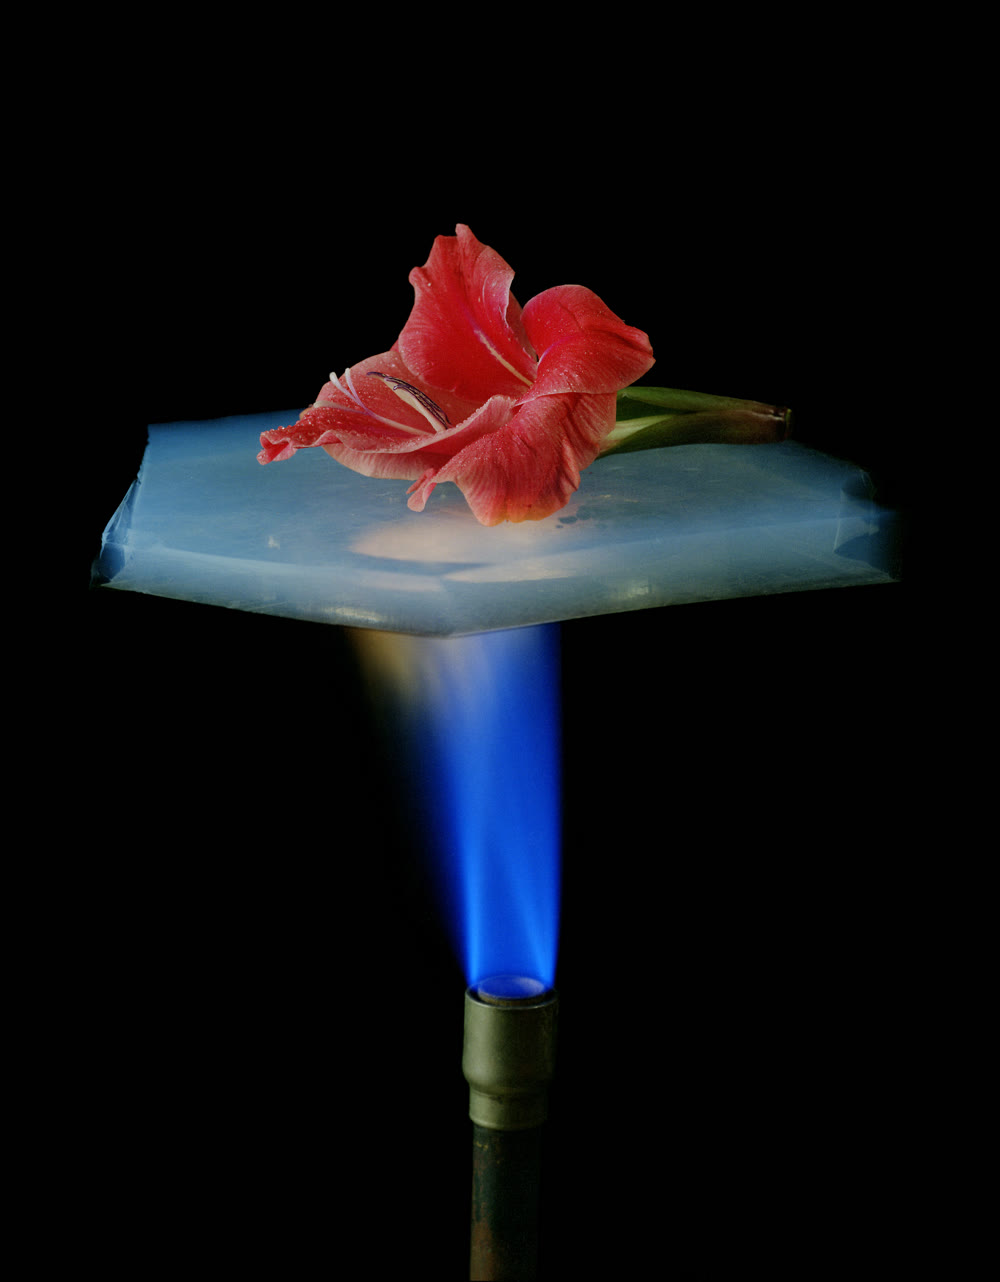
\includegraphics[width=0.38\linewidth]{images/book4/aerogel-flower.jpg}

{\small زهرة على لوح من \omterm{def:b3:colloids:colloid}{هلام} السيليكا الهوائي فوق لهب غاز: \omterm{def:b3:inorganic-materials:sol-gel}{فالهلام الهوائي}،
وهو \omterm{def:b3:colloids:colloid}{هلام} مجفف معظمه فراغ، رديء التوصيل للحرارة جدًا. الصورة:
ناسا/مختبر الدفع النفاث، ملكية عامة.}
\end{omfigure}

\section{طرق التخليق}

\begin{definition}[الطريقة الخزفية]\label{def:b3:inorganic-materials:ceramic-method}
\emph{الطريقة الخزفية}\index{طريقة خزفية} تصنع مركبًا صلبًا
بطحن المتفاعلات الصلبة معًا وتسخينها، أيامًا في الغالب ومع
إعادة الطحن، عند درجات حرارة مرتفعة بما يكفي لكي تنتشر الأيونات عبر
الصلبة.
\end{definition}

يجري تفاعل صلبين عند تماسهما، ويكوّن الناتج طبقة
بينهما يجب أن تعبرها الأيونات بعد ذلك: فأبطأ خطوة
هي الانتشار، وهو يتباطأ كلما ثخنت الطبقة.

\begin{proposition}[النمو القطعي المكافئ]\label{prop:b3:inorganic-materials:parabolic}
إذا كان نمو طبقة ناتج محدودًا بالانتشار عبرها، فإن
سمكها ينمو وفق $x^2 = kt$.
\end{proposition}

\begin{proof}
مع تراكيز ثابتة على وجهي الطبقة، يخضع التدفق عبرها
لقانون فيك، $J = D\Delta c/x$. وتنمو الطبقة بالتناسب مع التدفق:
$\dd x/\dd t = \lambda J = \lambda D\Delta c/x$، مع $\lambda$ حجم الناتج لكل مول منقول. ثم
$x\,\dd x = \lambda D\Delta c\,\dd t$، وبالمكاملة من $x = 0$ عند $t = 0$ نحصل على $x^2 = 2\lambda D\Delta c\,t = kt$.
\end{proof}

فمضاعفة حجم الجسيمات تضرب زمن التفاعل في أربعة: ومن هنا
الطحن الدقيق، أو الخلط على المستوى الذري في طليعة (\omterm{def:b3:colloids:colloid}{هلام} مختلط من الأكسالات أو
السترات يتفكك إلى المركب الهدف)، أو طريق في المحلول.

\begin{definition}[عملية الصول--الهلام]\label{def:b3:inorganic-materials:sol-gel}
\emph{عملية الصول--الهلام}\index{عملية الصول--الهلام} تصنع أكسيدًا
بحلمأة طلائع جزيئية، هي عادة ألكوكسيدات، وتكاثفها في
المحلول: فيصير المحلول صولًا من عناقيد أكسيدية صغيرة، ثم هلامًا، أي
شبكة صلبة متصلة مملوءة بالسائل. وإذا جُفف \omterm{def:b3:colloids:colloid}{الهلام} بالتبخير
انكمش إلى \emph{هلام جاف}\index{هلام جاف} كثيف؛ وإذا جُفف فوق النقطة
الحرجة للسائل، وهذا يزيله دون سطح فاصل بين سائل وغاز، احتفظ
بحجمه في صورة \emph{هلام هوائي}\index{هلام هوائي}.
\end{definition}

\begin{omfigure}
\setchemfig{atom sep=2.0em}
\schemestart
\chemfig{RO-Si(-[2]OR)(-[6]OR)-OR}
\+ \chemfig{H_2O}
\arrow{->[حلمأة]}[,1.4]
\chemfig{RO-Si(-[2]OR)(-[6]OR)-OH}
\+ ROH
\schemestop
\par\bigskip
\schemestart
\chemfig{{\equiv}Si-OH}
\+
\chemfig{HO-Si{\equiv}}
\arrow{->[تكاثف]}[,1.6]
\chemfig{{\equiv}Si-O-Si{\equiv}}
\+ \chemfig{H_2O}
\schemestop
\par\medskip

{\small كيمياء \omterm{def:b3:inorganic-materials:sol-gel}{الصول--الهلام} لألكوكسيد السيليكون (R: مجموعة ألكيل، إيثيل في
رباعي إيثيل أورثوسيليكات): يحل الماء محل مجموعات الألكوكسي بمجموعات هيدروكسي، 
ويتكاثف سيلانولان في جسر سيلوكسان. وبالتكرار، تبني التكاثفات
شبكة سيليكا ثلاثية الأبعاد.}
\end{omfigure}

يعطي التفاعلان معًا، من أجل تفاعل تام،
$\ce{Si(OC2H5)4 + 2H2O -> SiO2 + 4C2H5OH}$. والحفز الحمضي يجعل الحلمأة سريعة 
والتكاثف بطيئًا، فيعطي بوليمرات رقيقة شبيهة بالسلاسل؛ والحفز القاعدي يفعل
العكس، فيعطي جسيمات كثيفة. وتُصنع الطلاءات (طبقات مضادة للانعكاس على الزجاج)
بغمس القطعة في \omterm{def:b3:colloids:colloid}{الصول} وسحبها منه.

\begin{definition}[التخليق الحرمائي]\label{def:b3:inorganic-materials:hydrothermal}
\emph{التخليق الحرمائي}\index{تخليق حرمائي} يبلور
صلبًا من الماء فوق درجة غليانه العادية، في وعاء مغلق تحت
ضغط بخاره الذاتي؛ و\emph{التخليق الحرمذيبي}\index{تخليق حرمذيبي}
يفعل الشيء نفسه في مذيب آخر.
\end{definition}

\begin{definition}[الترسيب الكيميائي من البخار]\label{def:b3:inorganic-materials:cvd}
\emph{الترسيب الكيميائي من البخار}\index{ترسيب كيميائي من البخار} (CVD) يُنمي
غشاءً صلبًا على سطح مسخَّن بتفاعل طلائع غازية عليه، مثل
السيليكون من السيلان، $\ce{SiH4 -> Si + 2H2}$، أو الألماس من الميثان والهيدروجين.
\end{definition}

\begin{method}[اختيار طريق التخليق]\label{met:b3:inorganic-materials:route}
\begin{enumerate}
  \item أكسيد مستقر حراري في صورة مسحوق: \omterm{def:b3:inorganic-materials:ceramic-method}{الطريقة الخزفية}، مع
        طليعة إذا كان الخلط صعبًا.
  \item طور شبه مستقر، أو مسحوق دقيق أو طلاء عند درجة حرارة منخفضة:
        \omterm{def:b3:inorganic-materials:sol-gel}{الصول--الهلام} أو الترسيب من المحلول.
  \item بلورات أحادية كبيرة لطور لا يذوب إلا في الماء الساخن (الكوارتز) أو
        هيكل مبني حول قالب (الزيوليتات): \omterm{def:b3:inorganic-materials:hydrothermal}{التخليق الحرمائي}.
  \item غشاء رقيق نقي على ركيزة (طبقات أشباه الموصلات): \omterm{def:b3:inorganic-materials:cvd}{الترسيب الكيميائي من البخار}.
\end{enumerate}
\end{method}

\begin{inthelab}[طلاء بالصول--الهلام وأوتوكلاف]
يُحرَّك رباعي إيثيل أورثوسيليكات مع الإيثانول والماء وقطرة حمض
حتى يصفو المحلول؛ وتُغمس فيه شريحة زجاجية نظيفة وتُسحب
بسرعة بطيئة منتظمة، ثم تُجفف وتُسخَّن، فتبقى عليها طبقة سيليكا رقيقة بما يكفي
لإظهار ألوان التداخل. وفي \omterm{def:b3:inorganic-materials:hydrothermal}{التخليق الحرمائي} توضع المتفاعلات
في بطانة من البولي تترافلوروإيثيلين، لا تُملأ أكثر من نحو الثلثين كي
لا يملأ السائل المتمدد الوعاء، وتُختم في أوتوكلاف من الفولاذ
وتُسخَّن في فرن؛ ولا يُفتح الأوتوكلاف إلا بعد أن يبرد.
\end{inthelab}

\begin{omfigure}
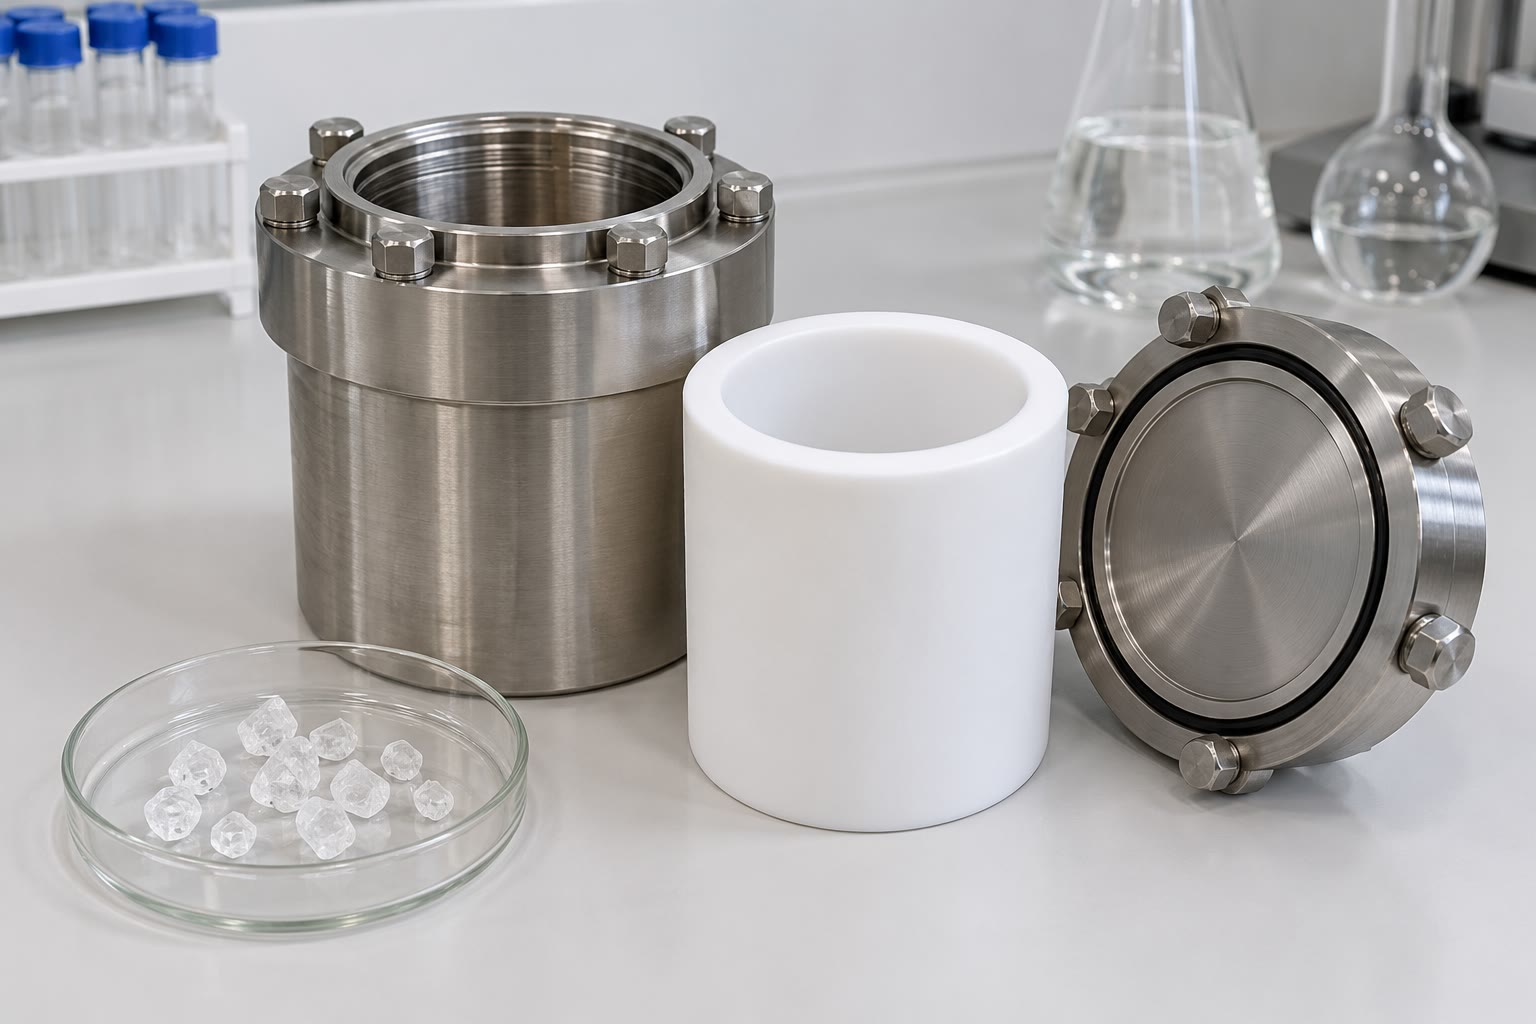
\includegraphics[width=0.5\linewidth]{images/book4/ai/b3-23-autoclave.jpg}

{\small أوتوكلاف مختبري \omterm{def:b3:inorganic-materials:hydrothermal}{للتخليق الحرمائي}: جسم من الفولاذ بغطاء
مثبَّت بالبراغي، وبطانة بوليمرية بيضاء تحوي مزيج التفاعل، وبلورات
نمت فيه.}
\end{omfigure}

\section{الخزفيات والزجاج}

\begin{definition}[الخزف]\label{def:b3:inorganic-materials:ceramic}
\emph{الخزف}\index{خزف} صلب غير عضوي وغير فلزي يُصنع
بتسخين مسحوق: أكاسيد ونتريدات وكربيدات، أو منتجات طينية.
\end{definition}

\begin{definition}[بنية البيروفسكيت]\label{def:b3:inorganic-materials:perovskite}
في \emph{بنية البيروفسكيت}\index{بنية البيروفسكيت} لأكسيد $\mathrm{ABO_3}$
تقع الكاتيونات B الصغيرة في مراكز ثمانيات أوجه $\mathrm{BO_6}$ مشتركة الرؤوس، 
والكاتيونات A الكبيرة في التجاويف الاثني عشرية التناسق بينها؛ وفي
الخلية المكعبة المثالية، يقع B في المركز، وO في مراكز الأوجه، وA في الرؤوس.
و\emph{عامل التسامح}\index{عامل التسامح} يقيس مدى توافق
الأيونات:
\[
  t = \frac{r_A + r_O}{\sqrt2\,(r_B + r_O)}.
\]
\end{definition}

\begin{omfigure}
\tdplotsetmaincoords{60}{100}
\begin{tikzpicture}[tdplot_main_coords, scale=1.5, font=\small,
  aA/.style={om atom, ball color=green!45!black, minimum size=7.4mm},
  aB/.style={om atom, ball color=black!35, minimum size=4.4mm},
  aOs/.style={om atom, ball color=red!80, minimum size=4.8mm}]
  \pic[transform shape] {omcubeo={2}};
  % atoms back to front for view 60/100 (depth 0.853x + 0.150y + 0.5z)
  \node[aA] at (0,0,0) {};
  \node[aA] at (0,2,0) {};
  \node[aOs] (o1) at (0,1,1) {};
  \node[aA] at (0,0,2) {};
  \node[aOs] (o2) at (1,1,0) {};
  \node[aA] at (0,2,2) {};
  \node[aOs] (o3) at (1,0,1) {};
  \node[aB] (b) at (1,1,1) {};
  \node[aOs] (o4) at (1,2,1) {};
  \node[aA] at (2,0,0) {};
  \node[aOs] (o5) at (1,1,2) {};
  \node[aA] at (2,2,0) {};
  \node[aOs] (o6) at (2,1,1) {};
  \node[aA] at (2,0,2) {};
  \node[aA] at (2,2,2) {};
  \begin{scope}[on background layer]
    \draw[omMeth!70, line width=0.6pt] (o1.center) -- (o2.center) -- (o6.center) -- (o5.center) -- cycle
      (o3.center) -- (o2.center) -- (o4.center) -- (o5.center) -- cycle
      (o1.center) -- (o3.center) -- (o6.center) -- (o4.center) -- cycle;
    \draw[bond] (b.center) -- (o1.center) (b.center) -- (o2.center) (b.center) -- (o3.center)
      (b.center) -- (o4.center) (b.center) -- (o5.center) (b.center) -- (o6.center);
  \end{scope}
  \node[anchor=west] at (2,3.35,2) {A};
  \node[anchor=west] at (2,3.35,1) {O};
  \node[anchor=west] at (2,3.35,0) {B};
  \node[aA, minimum size=4mm] at (2,3.2,2) {};
  \node[aOs, minimum size=3.2mm] at (2,3.2,1) {};
  \node[aB, minimum size=3mm] at (2,3.2,0) {};
\end{tikzpicture}

{\small خلية البيروفسكيت المكعبة $\mathrm{ABO_3}$: كاتيون B (رمادي) في مركز
ثماني أوجه من ستة أيونات أكسيد في مراكز الأوجه (الأحرف الخضراء)، والكاتيونات A
في الرؤوس. ويتقاسم كل أيون A في رأس ثماني خلايا ويتقاسم كل أكسجين
خليتان: أي A واحد وB واحد وثلاثة O في الخلية.}
\end{omfigure}

\begin{proposition}[عامل التسامح المثالي]\label{prop:b3:inorganic-materials:tolerance}
في البيروفسكيت المكعب المثالي، حيث تتلامس الأيونات على امتداد الاتجاهين B--O وA--O،
$t = 1$.
\end{proposition}

\begin{proof}
مع ضلع $a$، يبعد B في المركز وO في مركز وجه أحدهما عن الآخر $a/2$: $r_B + r_O = a/2$.
ويبعد A في رأس وO في مركز وجه مجاور نصف قطر
وجه: $r_A + r_O = a\sqrt2/2$. وبالقسمة، $(r_A + r_O)/(r_B + r_O) = \sqrt2$، ومنه $t = 1$.
\end{proof}

حين يكون $t$ أدنى من 1 بقليل، يكون الأيون A أصغر من تجويفه فتميل
ثمانيات الأوجه لتنغلق حوله، فتنخفض درجة التناظر؛ وحين يكون $t$ فوق 1،
يكون الأيون B أصغر من ثماني أوجهه فيمكن أن ينزاح عن المركز.

\begin{definition}[المادة الكهروحديدية]\label{def:b3:inorganic-materials:ferroelectric}
\emph{المادة الكهروحديدية}\index{مادة كهروحديدية} بلورة ذات استقطاب
كهربائي تلقائي يستطيع مجال كهربائي مطبَّق أن يعكسه.
\end{definition}

% ledger: rion:Ba2+XII, rion:Ti4+VI, rion:O2-VI
تيتانات الباريوم هي المثال الكلاسيكي: مع $r(\ce{Ba^2+}) = \qty{161}{pm}$ (تناسق اثنا عشري)،
و$r(\ce{Ti^4+}) = \qty{60.5}{pm}$ و$r(\ce{O^2-}) = \qty{140}{pm}$، يكون $t = 1.06$. ودون درجة حرارة تحول تنزاح
أيونات التيتانيوم عن المركز، كلها في الاتجاه نفسه داخل النطاق الواحد،
فتستقطب البلورة؛ والسماحية الهائلة قرب التحول تجعل
تيتانات الباريوم العازلَ الكهربائي في معظم المكثفات الخزفية.

\begin{definition}[الزجاج الأكسيدي]\label{def:b3:inorganic-materials:glass}
\emph{الزجاج الأكسيدي}\index{زجاج أكسيدي} صلب أكسيدي لابلوري، يُصنع
بتبريد مصهور دون تبلور. و\emph{مكوِّنات
الشبكة}\index{مكون الشبكة} فيه ($\ce{SiO2}$، $\ce{B2O3}$، $\ce{P2O5}$) تبني شبكة متصلة من
متعددات أوجه مشتركة الرؤوس؛ أما \emph{معدِّلات الشبكة}\index{معدل الشبكة}
($\ce{Na2O}$، $\ce{CaO}$) فتكسر جسورًا في تلك الشبكة، إذ يحوّل كل أيون أكسيد يضاف
أكسجينًا جسريًا واحدًا إلى أكسجينين غير جسريين، وتجلس الكاتيونات في
الفجوات.
\end{definition}

\begin{omfigure}
\begin{tikzpicture}
\begin{axis}[name=c, width=0.5\linewidth, axis equal image, hide axis, xmin=-1.2, xmax=12.6, ymin=-1.2, ymax=8.7]
\addplot[quiver={u=\thisrow{u}, v=\thisrow{v}}, -, black!60, line width=0.6pt] table {figdata/out/bachelor-3-glass-network-crystal-bonds.dat};
\addplot[only marks, mark=*, mark size=2.2pt, omDef] table {figdata/out/bachelor-3-glass-network-crystal-T.dat};
\addplot[only marks, mark=*, mark size=1.3pt, omThm, mark options={fill=white}] table {figdata/out/bachelor-3-glass-network-crystal-O.dat};
\end{axis}
\begin{axis}[at={(c.east)}, anchor=west, xshift=0.2cm, width=0.5\linewidth, axis equal image, hide axis, xmin=-1.2, xmax=12.6, ymin=-1.2, ymax=8.7]
\addplot[quiver={u=\thisrow{u}, v=\thisrow{v}}, -, black!60, line width=0.6pt] table {figdata/out/bachelor-3-glass-network-glass-bonds.dat};
\addplot[only marks, mark=*, mark size=2.2pt, omDef] table {figdata/out/bachelor-3-glass-network-glass-T.dat};
\addplot[only marks, mark=*, mark size=1.3pt, omThm, mark options={fill=white}] table {figdata/out/bachelor-3-glass-network-glass-O.dat};
\addplot[only marks, mark=*, mark size=1.5pt, omThm] table {figdata/out/bachelor-3-glass-network-glass-NBO.dat};
\addplot[only marks, mark=*, mark size=2.6pt, omProp] table {figdata/out/bachelor-3-glass-network-glass-Na.dat};
\end{axis}
\end{tikzpicture}

{\small صورة ثنائية الأبعاد لبلورة ولزجاج من
التركيب نفسه (بالأزرق: مكوِّنات ثلاثية التناسق؛ دوائر حمراء مفتوحة: ذرات أكسجين
جسرية). يسارًا، تكرر البلورة حلقة واحدة. يمينًا، الزجاج: فكل مكوِّن
لا يزال حوله ثلاث ذرات أكسجين على المسافات نفسها تقريبًا، لكن للحلقات خمسة أو
ستة أو سبعة أعضاء ولا شيء يتكرر؛ وفي موضعين كسر معدِّلٌ
جسرًا، تاركًا ذرتي أكسجين غير جسريتين (حمراوين ممتلئتين) وكاتيونًا (برتقاليًا) في
الفجوة. شبكة نموذجية، أُرخيت بالنوابض.}
\end{omfigure}

رأى ويليام زاكارياسن في سنة 1932 أن الأكسيد يكوّن زجاجًا بسهولة حين يكون
كاتيونه محاطًا بقليل من ذرات الأكسجين (ثلاث أو أربع)، وتربط كل ذرة أكسجين
كاتيونين على الأكثر، وتشترك متعددات الأوجه في الرؤوس، لا في الأحرف أو الأوجه: عندئذ
لا تكلّف الشبكة العشوائية طاقة أكثر من البلورة إلا قليلًا. وزجاج النوافذ
سيليكا مع أكسيدي الصوديوم والكالسيوم معدِّلين، يخفضان درجة حرارة
الانصهار. ويُغمس زجاج الهواتف المقسّى في نترات البوتاسيوم
المصهورة: فتحل أيونات $\ce{K+}$ الأكبر محل أيونات $\ce{Na+}$ في السطح، ولأنها مزدحمة،
تضعه تحت الانضغاط، فلا تنفتح الشقوق.

\section{الصلبة المسامية: الزيوليتات والأطر}

\begin{definition}[الزيوليتات]\label{def:b3:inorganic-materials:zeolite}
\emph{الزيوليت}\index{زيوليت} ألومينوسيليكات بلورية يحيط
هيكلها المكوّن من رباعيات أوجه $\ce{SiO4}$ و$\ce{AlO4}$ مشتركة الرؤوس بأقفاص 
وقنوات بحجم الجزيئات، فيها كاتيونات قابلة للتبادل وماء. 
و\emph{المنخل الجزيئي}\index{منخل جزيئي} صلب مسامي يُدخل
الجزيئات بحسب حجمها؛ و\emph{الانتقائية الشكلية}\index{انتقائية شكلية}
هي التحكم في تفاعل بحجم المسام التي يجري فيها وشكلها.
\end{definition}

يحمل كل رباعي أوجه $\ce{AlO4}$ شحنة سالبة واحدة زيادةً على $\ce{SiO4}$
(الألومنيوم(III) مكان السيليكون(IV))؛ وتوازنها الكاتيونات في الأقفاص، $\ce{Na+}$ أو $\ce{Ca^2+}$،
ويمكن تبادلها.

\begin{proposition}[قاعدة لوفنشتاين]\label{prop:b3:inorganic-materials:lowenstein}
في هيكل \omterm{def:b3:inorganic-materials:zeolite}{زيوليت} لا يشترك رباعيا أوجه $\ce{AlO4}$ أبدًا في ذرة أكسجين: فالروابط Al--O--Al
غائبة (وهذه ملاحظة على كل هياكل الألومينوسيليكات المعروفة). 
ونتيجةً لذلك تكون النسبة Si/Al في \omterm{def:b3:inorganic-materials:zeolite}{الزيوليت} 1 على الأقل.
\end{proposition}

\begin{proof}[برهان النتيجة]
لكل ذرة ألومنيوم أربع ذرات أكسجين، تتقاسم كلًّا منها مع ذرة سيليكون بحكم القاعدة:
أي $4N_{\mathrm{Al}}$ رابطة Al--O--Si. ولكل ذرة سيليكون أربع ذرات أكسجين فقط، فلا تشارك إلا في
أربع روابط من هذا النوع على الأكثر: $4N_{\mathrm{Al}} \le 4N_{\mathrm{Si}}$، أي $N_{\mathrm{Si}}/N_{\mathrm{Al}} \ge 1$. والمساواة تفرض أن يكون لكل
ذرة سيليكون أربعة جيران من الألومنيوم: فيتناوب Si وAl.
\end{proof}

\begin{omfigure}
\tdplotsetmaincoords{55}{135}
\begin{tikzpicture}[tdplot_main_coords, scale=0.85, font=\small, baseline=(current bounding box.center),
  tSi/.style={circle, inner sep=0pt, minimum size=2.6mm, draw=black!70, fill=omDef!80},
  tAl/.style={circle, inner sep=0pt, minimum size=2.6mm, draw=black!70, fill=omProp!80}]
  % edges of a truncated octahedron (vertices: permutations of (0, +-1, +-2));
  % hidden edges (both faces facing away for this view) dashed
  \foreach \a/\b/\c/\d/\e/\f in {-2/-1/0/-2/0/-1, -2/-1/0/-2/0/1, -2/-1/0/-1/-2/0, -2/0/-1/-2/1/0, -2/0/-1/-1/0/-2, -1/-2/0/0/-2/-1, -1/-2/0/0/-2/1, -1/0/-2/0/-1/-2, -1/0/-2/0/1/-2, 0/-2/-1/0/-1/-2, 0/-2/-1/1/-2/0, 0/-1/-2/1/0/-2}
    \draw[black!40, dashed] (\a,\b,\c) -- (\d,\e,\f);
  \foreach \a/\b/\c/\d/\e/\f in {-2/0/1/-2/1/0, -2/0/1/-1/0/2, -2/1/0/-1/2/0, -1/0/2/0/-1/2, -1/0/2/0/1/2, -1/2/0/0/2/-1, -1/2/0/0/2/1, 0/-2/1/0/-1/2, 0/-2/1/1/-2/0, 0/-1/2/1/0/2, 0/1/-2/0/2/-1, 0/1/-2/1/0/-2, 0/1/2/0/2/1, 0/1/2/1/0/2, 0/2/-1/1/2/0, 0/2/1/1/2/0, 1/-2/0/2/-1/0, 1/0/-2/2/0/-1, 1/0/2/2/0/1, 1/2/0/2/1/0, 2/-1/0/2/0/-1, 2/-1/0/2/0/1, 2/0/-1/2/1/0, 2/0/1/2/1/0}
    \draw[black!75, line width=0.7pt] (\a,\b,\c) -- (\d,\e,\f);
  % T atoms back to front; hidden ones paler
  \foreach \x/\y/\z/\k/\v in {-2/-1/0/Si/0, -1/-2/0/Al/0, -2/0/-1/Al/0, 0/-2/-1/Si/0, -1/0/-2/Si/0, 0/-1/-2/Al/0, -2/0/1/Al/1, 0/-2/1/Si/1, -2/1/0/Si/1, 1/-2/0/Al/1, 0/1/-2/Al/1, 1/0/-2/Si/1, -1/0/2/Si/1, 0/-1/2/Al/1, -1/2/0/Al/1, 2/-1/0/Si/1, 0/2/-1/Si/1, 2/0/-1/Al/1, 0/1/2/Al/1, 1/0/2/Si/1, 0/2/1/Si/1, 2/0/1/Al/1, 1/2/0/Al/1, 2/1/0/Si/1}
    \node[t\k, opacity=0.35+0.65*\v] at (\x,\y,\z) {};
\end{tikzpicture}
\hspace{1.2cm}
\begin{tikzpicture}[font=\small, scale=0.8, baseline=(current bounding box.center)]
  \foreach \i in {0,1,2} \foreach \j in {0,1,2} {
    \fill[omDef!70] ($(2.2*\i,2.2*\j)+(-0.28,-0.28)$) rectangle +(0.56,0.56);
  }
  \foreach \i in {0,1} \foreach \j in {0,1,2} {
    \draw[black!70, line width=0.8pt] (2.2*\i+0.28,2.2*\j) -- (2.2*\i+0.75,2.2*\j);
    \draw[black!70, line width=0.8pt] (2.2*\i+1.45,2.2*\j) -- (2.2*\i+1.92,2.2*\j);
    \node[draw=black!70, regular polygon, regular polygon sides=6, minimum size=5.6mm, inner sep=0pt] at (2.2*\i+1.1,2.2*\j) {};
  }
  \foreach \i in {0,1,2} \foreach \j in {0,1} {
    \draw[black!70, line width=0.8pt] (2.2*\i,2.2*\j+0.28) -- (2.2*\i,2.2*\j+0.75);
    \draw[black!70, line width=0.8pt] (2.2*\i,2.2*\j+1.45) -- (2.2*\i,2.2*\j+1.92);
    \node[draw=black!70, regular polygon, regular polygon sides=6, minimum size=5.6mm, inner sep=0pt] at (2.2*\i,2.2*\j+1.1) {};
  }
  \node[font=\scriptsize, align=center] at (1.1,-0.85) {\foreignlanguage{arabic}{عقدة $\ce{Zn4O}$ $+$ رابط تيريفثالات}};
\end{tikzpicture}

{\small يسارًا: قفص سودالايت، وحدة بناء \omterm{def:b3:inorganic-materials:zeolite}{الزيوليت} A، مع
ذرة رباعية التناسق في كل رأس (وذرات الأكسجين، في منتصف كل حرف، غير
مرسومة)؛ ويتناوب السيليكون (بالأزرق) والألومنيوم (بالبرتقالي)، كما تقتضي قاعدة لوفنشتاين
حين Si/Al = 1. يمينًا: طبقة من \omterm{def:b3:inorganic-materials:mof}{إطار فلزي عضوي}،
رسم تخطيطي: عناقيد $\ce{Zn4O}$ (المربعات) تربطها روابط بنزين-1،4-ثنائي الكربوكسيلات
(الحلقات) في شبكة مكعبة ذات \omterm{def:b3:inorganic-materials:pores}{مسام كبيرة}.}
\end{omfigure}

\begin{method}[صيغة الزيوليت وسعته التبادلية]\label{met:b3:inorganic-materials:zeolite-formula}
\begin{enumerate}
  \item اكتب الهيكل في الصورة $\mathrm{[(AlO_2)_x(SiO_2)_y]^{x-}}$: Si/Al $= y/x$.
  \item توازن الكاتيوناتُ شحنةَ الهيكل $-x$: أي $x$ كاتيونًا أحادي الشحنة أو $x/2$
        كاتيونًا ثنائي الشحنة.
  \item السعة التبادلية هي كمية الشحنة القابلة للتبادل لكل غرام:
        $x/M$ مول من الكاتيونات الأحادية الشحنة، و$x/2M$ من الثنائية الشحنة، مع $M$
        الكتلة المولية للصيغة كما توزن (لامائية أو مميَّهة).
\end{enumerate}
\end{method}

\begin{proposition}[السعة التبادلية]\label{prop:b3:inorganic-materials:exchange-capacity}
سعة \omterm{def:b3:inorganic-materials:zeolite}{زيوليت} إزاء كاتيون شحنته $z$ هي $x/(zM)$ مول لكل غرام،
حيث $x$ عدد ذرات الألومنيوم في صيغة كتلتها المولية $M$.
\end{proposition}

\begin{proof}
تسهم كل ذرة ألومنيوم بشحنة سالبة واحدة في الهيكل؛ ويقتضي التعادل
الكهربائي $x$ وحدة من الشحنة الموجبة، كلها قابلة للتبادل، أي
$x/z$ كاتيونًا شحنته $z$ لكل وحدة صيغية، أي لكل كتلة $M$.
\end{proof}

% ledger: iza:LTA.window, iza:MFI.channels
\omterm{def:b3:inorganic-materials:zeolite}{للزيوليت} A نوافذ من ثمانية رباعيات أوجه، قطرها \qty{0.41}{nm}: فيمر منها الماء 
والأيونات الصغيرة، ولا تمر الجزيئات المتفرعة. وللزيوليت ZSM-5 مجموعتان من القنوات من عشرة
رباعيات أوجه، نحو 0.51 إلى \qty{0.56}{nm}: ففي تحويل الميثانول أو
ألكلة التولوين، ينتشر \textit{para}-زيلين النحيل إلى الخارج أسرع بكثير من
متماكبيه \textit{ortho} و\textit{meta}، اللذين يبقيان ويتماكبان. وهذه هي \omterm{def:b3:inorganic-materials:zeolite}{الانتقائية
الشكلية}.

\begin{definition}[الأطر الفلزية العضوية]\label{def:b3:inorganic-materials:mof}
\emph{الإطار الفلزي العضوي}\index{إطار فلزي عضوي} (MOF)
صلب بلوري مبني من أيونات فلزية أو عناقيد تربطها روابط
عضوية متعددة المواضع في شبكة مسامية. و\emph{وحدة البناء
الثانوية}\index{وحدة البناء الثانوية} هي العنقود الفلزي مع
مجموعاته التناسقية، معامَلًا على أنه عقدة واحدة في الشبكة؛ و\emph{التخليق
الشبكي}\index{تخليق شبكي} هو تصميم إطار باختيار
عُقد وروابط ذات هندسة معينة بحيث تتجمع في شبكة مختارة.
\end{definition}

% ledger: cod:MOF5.formula, cod:MOF5.a
في MOF-5، تكون عناقيد $\ce{Zn4O}$ ذات مجموعات الكربوكسيلات الست عقدًا ثمانية الأوجه،
وتربطها روابط بنزين-1،4-ثنائي الكربوكسيلات على امتداد أحرف شبكة
مكعبة، $a = \qty{25.82}{\angstrom}$ لخلية من ثماني عقد. واستبدال الرابط برابط أطول
يحفظ الشبكة ويوسع المسام: وهذه هي الفكرة الشبكية. ولهذه
الأطر مساحات سطحية تبلغ آلاف الأمتار المربعة لكل غرام، وتُدرس
لتخزين الهيدروجين والميثان ولالتقاط ثنائي أكسيد الكربون.

\begin{definition}[أحجام المسام]\label{def:b3:inorganic-materials:pores}
% ledger: pore:micro, pore:macro
اصطلاحًا، \emph{المسام الدقيقة}\index{مسام دقيقة} أضيق من \qty{2}{nm}،
و\emph{المسام المتوسطة}\index{مسام متوسطة} بين 2 و\qty{50}{nm}، 
و\emph{المسام الكبيرة}\index{مسام كبيرة} أعرض من \qty{50}{nm}.
\end{definition}

الزيوليتات ومعظم الأطر الفلزية العضوية دقيقة المسام؛ وهلامات السيليكا والهلامات الهوائية متوسطة المسام.

\section{الجسيمات النانوية}

\begin{definition}[المواد النانوية]\label{def:b3:inorganic-materials:nano}
\emph{المادة النانوية}\index{مادة نانوية} لها بُعد واحد على الأقل بين
نحو 1 و\qty{100}{nm}؛ و\emph{الجسيم النانوي}\index{جسيم نانوي} له
الأبعاد الثلاثة كلها في هذا المجال.
\end{definition}

\begin{proposition}[العناقيد السحرية]\label{prop:b3:inorganic-materials:magic}
العنقود المكعب الثماني الأوجه المكوَّن من ذرة مركزية و$n$ قشرة كاملة فيه
\[
  N(n) = \frac{10n^3 + 15n^2 + 11n + 3}{3}
\]
ذرة، منها $10n^2 + 2$ على السطح: 13، 55، 147، 309، \dots
\end{proposition}

\begin{proof}
للقشرة رقم $k$ في المكعب الثماني الأوجه 12 رأسًا، و24 حرفًا في داخل كل منها $k - 1$ ذرة،
و8 أوجه مثلثية في كل منها $(k - 1)(k - 2)/2$ ذرة داخلية و6
أوجه مربعة في كل منها $(k - 1)^2$: والمجموع $12 + 24(k - 1) + 4(k - 1)(k - 2) + 6(k - 1)^2 = 10k^2 + 2$. ثم
$N(n) = 1 + \sum_{k=1}^{n}(10k^2 + 2) = 1 + \frac{10n(n + 1)(2n + 1)}{6} + 2n$، وبالنشر نحصل على الصيغة؛ 
والقشرة الخارجية، $10n^2 + 2$ ذرة، هي السطح.
\end{proof}

\begin{omfigure}
\begin{tikzpicture}
\begin{axis}[name=a, width=0.47\linewidth, height=5.4cm, xmin=0, xmax=18, ymin=0, ymax=1,
  axis lines=left, xlabel={\foreignlanguage{arabic}{القطر \babelsublr{(\unit{nm})}}}, ylabel={\foreignlanguage{arabic}{نسبة الذرات على السطح}},
  tick label style={font=\scriptsize}, label style={font=\small}]
\addplot[omDef, thick, mark=*, mark size=1pt] table[x=diam_nm, y=fsurf] {figdata/out/bachelor-3-nanoparticle-size.dat};
\end{axis}
\begin{axis}[at={(a.east)}, anchor=west, xshift=1.5cm, width=0.47\linewidth, height=5.4cm,
  xmin=0.8, xmax=6, ymin=0, ymax=3, axis lines=left,
  xlabel={\foreignlanguage{arabic}{نصف القطر $R$ \babelsublr{(\unit{nm})}}}, ylabel={\foreignlanguage{arabic}{طاقة الحصر \babelsublr{(\unit{eV})}}},
  tick label style={font=\scriptsize}, label style={font=\small}]
\addplot[omThm, thick] table[x=R_nm, y=dE_eV] {figdata/out/bachelor-3-nanoparticle-size-b.dat};
\end{axis}
\end{tikzpicture}

{\small يسارًا: نسبة الذرات على سطح عناقيد الذهب المكعبة الثمانية الأوجه
بدلالة قطرها: أكثر من النصف في العناقيد الأصغر من نحو
\qty{3}{nm}، ولا تزال الخُمس عند \qty{8}{nm}. يمينًا: طاقة الحصر لزوج
إلكترون--ثقب في \omterm{def:b3:inorganic-materials:quantum-dot}{نقطة كمومية} كروية (\omterm{def:b3:quantum-model-systems:oscillator}{كتلة مختزلة} نموذجية $0.10\,m_e$)،
التي تضاف إلى \omterm{def:b3:solid-state:band}{الفجوة الحزمية} وتتناقص وفق $1/R^2$.}
\end{omfigure}

لما كان جزء كبير من ذرات \omterm{def:b3:inorganic-materials:nano}{الجسيم النانوي} على السطح، حيث يقل عدد
جيرانها، فإنه ينصهر عند درجة حرارة أدنى من الفلز الكتلي،
ويكون أكثر تفاعلية، وقد يكون حفازًا أفضل بكثير: فالذهب الكتلي خامل، أما جسيمات
الذهب التي يبلغ قطرها بضعة نانومترات فتؤكسد أحادي أكسيد الكربون في درجة حرارة الغرفة.

\begin{definition}[النقاط الكمومية]\label{def:b3:inorganic-materials:quantum-dot}
\emph{النقطة الكمومية}\index{نقطة كمومية} بلورة نانوية من \omterm{def:b3:solid-state:classes}{شبه موصل} صغيرة
بما يكفي لكي يرفع حصر إلكتروناتها وثقوبها فجوتها الحزمية
فوق فجوة الصلب الكتلي.
\end{definition}

\begin{theorem}[الحصر في كرة]\label{thm:b3:inorganic-materials:quantum-dot}
لجسيم كتلته $m$ محصور في كرة نصف قطرها $R$ بجدران لانهائية
طاقة الحالة الأساسية $E = \hbar^2\pi^2/(2mR^2) = h^2/(8mR^2)$، والدالة الموجية $\psi \propto \sin(\pi r/R)/r$.
\end{theorem}

\begin{proof}
من أجل حالة متناظرة كرويًا $\psi(r) = u(r)/r$، يعطي اللابلاسي
$\nabla^2\psi = u''/r$، فتصير \omterm{thm:b3:quantum-model-systems:schrodinger}{معادلة شرودنغر} في الداخل $-\frac{\hbar^2}{2m}u'' = Eu$، وهي معادلة جسيم على
خط. والحل الذي تكون فيه $\psi$ منتهية في المركز يحقق $u(0) = 0$: $u = \sin(kr)$، مع $E = \hbar^2k^2/2m$.
ويقتضي الجدار $u(R) = 0$، ومنه $kR = \pi$ للحالة الأساسية، و$E = \hbar^2\pi^2/(2mR^2)$.
\end{proof}

في \omterm{def:b3:inorganic-materials:quantum-dot}{النقطة الكمومية} يكون الإلكترون \omterm{def:b3:solid-state:carriers}{والثقب} كلاهما محصورين؛ وطاقة
أدنى إثارة هي $E_g + h^2/(8\mu R^2)$ في تقريب أول، مع $\mu$ كتلتهما
المختزلة (وتجاذب كولوم بينهما يخفضها قليلًا). وتنصيف نصف القطر
يضرب طاقة الحصر في أربعة: فنقاط سيلينيد الكادميوم التي يبلغ قطرها بضعة
نانومترات تتوهج بالأحمر أو الأخضر أو الأزرق بحسب حجمها وحده، وتُستعمل
بواعثَ في الشاشات.

\begin{definition}[رنين البلازمون السطحي]\label{def:b3:inorganic-materials:plasmon}
\emph{رنين البلازمون السطحي}\index{رنين البلازمون السطحي}
اهتزاز جماعي لإلكترونات التوصيل في جسيم فلزي نانوي
يقوده الضوء؛ ويعطي حزمة امتصاص قوية يتوقف طول موجتها على
الفلز، وعلى حجم الجسيم وشكله وعلى محيطه.
\end{definition}

جسيمات الذهب النانوية التي يبلغ قطرها بضع عشرات من النانومترات تمتص الضوء الأخضر وتبدو
حمراء ياقوتية في الزجاج أو في \omterm{def:b3:colloids:colloid}{غرواني}؛ وحين تتجمع، تنزاح الحزمة نحو
الأطوال الموجية الأطول ويصير اللون أزرق: وهذا أساس كثير من الاختبارات السريعة، التي
يتجمع فيها \omterm{def:b3:colloids:colloid}{غرواني} ذهب مكسو بأجسام مضادة في خط ملوّن.

\section{المواد النانوية الكربونية}

\begin{definition}[المواد النانوية الكربونية]\label{def:b3:inorganic-materials:carbon}
\emph{الفوليرين}\index{فوليرين} جزيء على شكل قفص مغلق من ذرات الكربون،
ترتبط كل منها بثلاث ذرات أخرى، بحلقات خماسية وسداسية، مثل
$\ce{C60}$ العشروني الأوجه. و\emph{الأنبوب الكربوني النانوي}\index{أنبوب كربوني نانوي} صفيحة من
الغرافيت ملفوفة في أسطوانة بلا درز قطرها نحو نانومتر.
و\emph{الغرافين}\index{غرافين} طبقة واحدة من الغرافيت، سمكها ذرة واحدة.
\end{definition}

\begin{proposition}[الخماسيات الاثنا عشر]\label{prop:b3:inorganic-materials:euler}
لكل \omterm{def:b3:inorganic-materials:carbon}{فوليرين} اثنا عشر خماسيًا بالضبط، مهما كان عدد
سداسياته.
\end{proposition}

\begin{proof}
القفص المغلق متعدد أوجه: فتصح صيغة أويلر $V - E + F = 2$. لكل ذرة
ثلاث روابط ولكل رابطة ذرتان: $2E = 3V$. ومع $p$ خماسيًا و$h$ سداسيًا،
يعطي عدّ الأحرف بالأوجه $2E = 5p + 6h$، و$F = p + h$. ثم $V = 2E/3$ وتصير صيغة
أويلر $-E/3 + p + h = 2$، أي $-(5p + 6h)/6 + p + h = 2$، ومنه $p/6 = 2$: $p = 12$.
\end{proof}

\begin{omfigure}
\begin{tikzpicture}[scale=0.62, font=\small]
  \def\hexd{0.6}
  \begin{scope}
    \clip (-0.4,-0.5) rectangle (9.6,5.2);
    \foreach \i in {-3,...,10} \foreach \j in {-1,...,6} {
      \pgfmathsetmacro\cx{1.7320508*\hexd*(\i + 0.5*\j)}
      \pgfmathsetmacro\cy{1.5*\hexd*\j}
      \draw[black!45] ({\cx+\hexd*cos(30)},{\cy+\hexd*sin(30)})
        \foreach \k in {90,150,...,390} { -- ({\cx+\hexd*cos(\k)},{\cy+\hexd*sin(\k)}) };
    }
  \end{scope}
  \draw[->, thick, omDef] (0,0) -- ({1.7320508*\hexd},0) node[below right, font=\scriptsize, fill=white, inner sep=1pt] {$\mathbf a_1$};
  \draw[->, thick, omDef] (0,0) -- ({1.7320508*\hexd*0.5},{1.5*\hexd}) node[left, font=\scriptsize, fill=white, inner sep=1pt] {$\mathbf a_2$};
  \draw[->, very thick, omThm] (0,0) -- ({1.7320508*\hexd*(4+0.5*2)},{1.5*\hexd*2}) node[above right, font=\scriptsize, fill=white, inner sep=1pt] {$\mathbf C_h = 4\mathbf a_1 + 2\mathbf a_2$};
  \draw[dashed, omMeth, thick] (0,0) -- ({1.7320508*\hexd*9},0) node[right, font=\scriptsize] {\foreignlanguage{arabic}{متعرج $(n, 0)$}};
  \draw[dashed, omProp, thick] (0,0) -- ({1.7320508*\hexd*5*1.5},{1.5*\hexd*5}) node[below right, font=\scriptsize, fill=white, inner sep=1pt] {\foreignlanguage{arabic}{كرسي $(n, n)$}};
\end{tikzpicture}

{\small صفيحة \omterm{def:b3:inorganic-materials:carbon}{غرافين} والمتجه الكيرالي لأنبوب نانوي: لفّ الصفيحة
بحيث يلتقي رأس $\mathbf C_h = n\mathbf a_1 + m\mathbf a_2$ بمبدئه يعطي الأنبوب $(n, m)$، وهو هنا $(4, 2)$.
وعلى امتداد $\mathbf a_1$ تكون حافة الأنبوب $(n, 0)$ متعرجة؛ وعلى امتداد $\mathbf a_1 + \mathbf a_2$، بزاوية 30°، تكون حافة الأنبوب $(n, n)$
على شكل كرسي.}
\end{omfigure}

\begin{proposition}[الأنابيب النانوية الفلزية وشبه الموصلة]\label{prop:b3:inorganic-materials:nanotube}
يكون \omterm{def:b3:inorganic-materials:carbon}{الأنبوب الكربوني النانوي} الأحادي الجدار $(n, m)$ فلزيًا حين يكون $n - m$ مضاعفًا للعدد 3، 
\omterm{def:b3:solid-state:classes}{وشبه موصل} فيما عدا ذلك. \admitted
\end{proposition}

فثلث الأنابيب الممكنة كلها فلزي إذن، ومن بينها كل الأنابيب
ذات حافة الكرسي؛ وفجوة الأخرى تتناقص كلما كبر قطرها. وليس \omterm{def:b3:inorganic-materials:carbon}{للغرافين} نفسه
أي فجوة: فحزمتا التكافؤ والتوصيل فيه تتلامسان في نقاط مفردة، 
وتتحرك إلكتروناته كأنها بلا كتلة.

\begin{safety}{\ghs[0.62cm]{GHS02}\ghs[0.62cm]{GHS07}\ghs[0.62cm]{GHS08}}
% ledger: ghs4:TEOS
رباعي إيثيل أورثوسيليكات: سائل وبخار قابلان للاشتعال، ضار إذا استُنشق،
مهيج للعينين والمسالك التنفسية؛ يُتداول تحت ساحبة الأبخرة. المساحيق النانوية:
تبلغ أدق الجسيمات أعماق الرئتين، وكثير منها لم يُصنَّف بعد؛
فتوزن وتُتداول في حيّز مغلق أو في صورة معلَّق، ولا تُتداول أبدًا في صورة
غبار سائب في الهواء الطلق.
\end{safety}

\begin{omfigure}
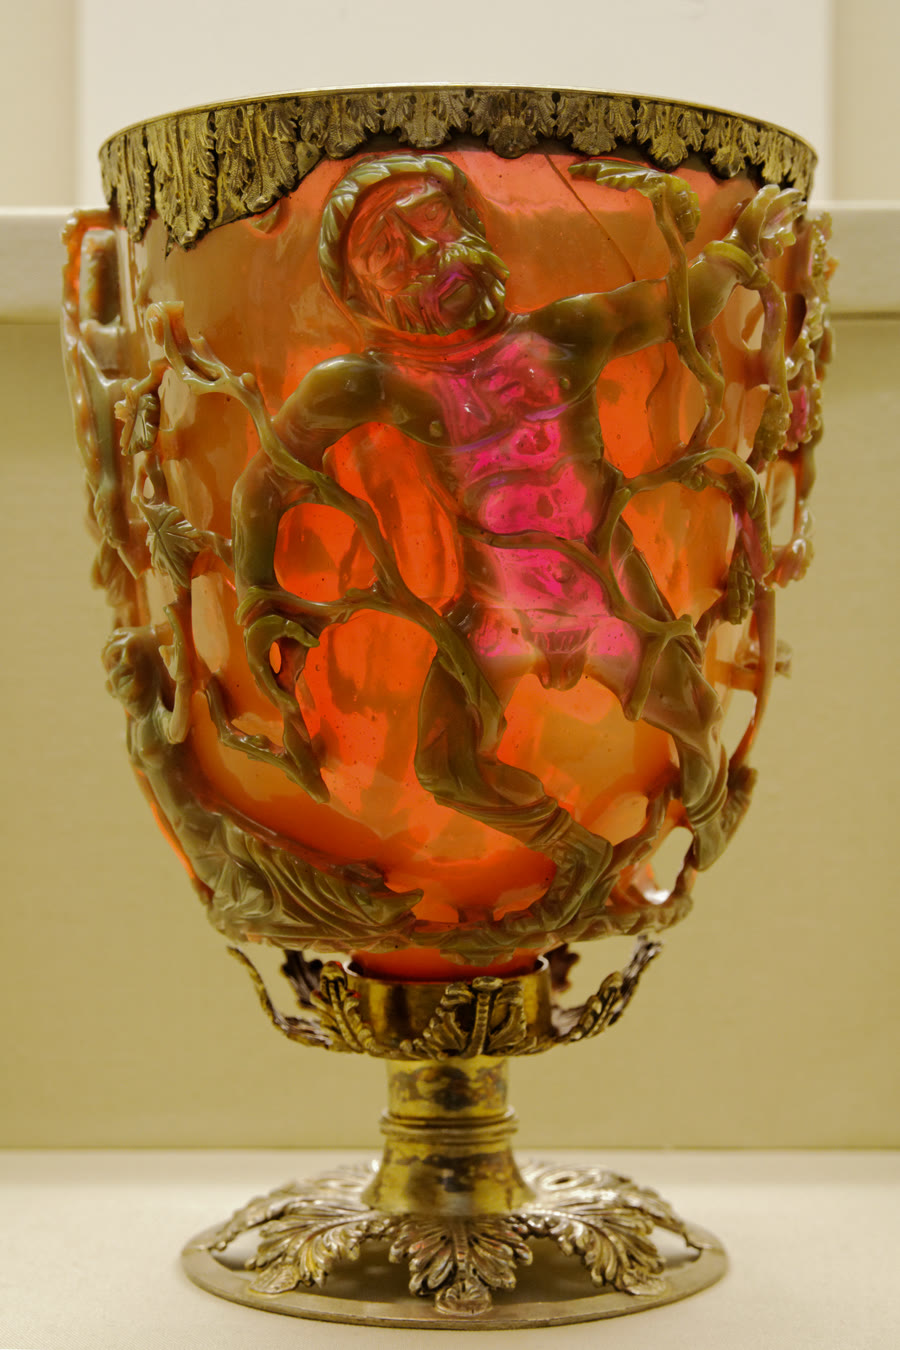
\includegraphics[width=0.32\linewidth]{images/book4/lycurgus-cup.jpg}

{\small كأس ليكورغوس، وهي آنية زجاجية رومانية من القرن الرابع، مضاءة من الداخل:
تبدو خضراء في الضوء المنعكس وحمراء في الضوء النافذ، وهذا أثر
\omterm{def:b3:inorganic-materials:nano}{جسيمات نانوية} من الذهب والفضة في الزجاج. الصورة: ماري-لان نغوين، CC BY
2.5.}
\end{omfigure}

\begin{history}[جسيمات نانوية قبل الكلمة، وكرة قدم من الكربون]
لوّن صانعو الزجاج الزجاجَ بالأحمر بالذهب قبل أن يعرف أحد السبب بزمن طويل؛ 
وتُظهر كأس ليكورغوس هذا الأثر في أروع صوره. وصنع مايكل فاراداي غرويات
الذهب في خمسينيات القرن التاسع عشر ورأى أن لونها يأتي من جسيمات أصغر من أن
تُرى. وفي سنة 1985 وجد هارولد كروتو وروبرت كيرل وريتشارد سمولي، وهم يبخّرون
الغرافيت بالليزر، أن عناقيد من ستين ذرة كربون مستقرة
استقرارًا استثنائيًا، واقترحوا القفص المغلق ذا الخماسيات الاثني عشر 
والسداسيات العشرين؛ ونالوا جائزة نوبل في الكيمياء لسنة 1996.
\end{history}

\section{تمارين}

\begin{exercise}[$\star$]\label{exo:b3:inorganic-materials:1}
طبقة ناتج بين صلبين سمكها \qty{2.0}{\micro\metre} بعد \qty{10}{h}. كم من الوقت يلزم حتى
يبلغ سمكها \qty{6.0}{\micro\metre}، إذا كان النمو قطعيًا مكافئًا؟
\end{exercise}

\begin{exercise}[$\star$]\label{exo:b3:inorganic-materials:2}
اكتب حلمأة رباعي إيثيل أورثوسيليكات إلى حمض السيليسيك، 
وتكاثف جزيئين من حمض السيليسيك، والتفاعل الإجمالي المعطي
للسيليكا.
\end{exercise}

\begin{exercise}[$\star$]\label{exo:b3:inorganic-materials:3}
صنّف $\ce{SiO2}$ و$\ce{B2O3}$ و$\ce{Na2O}$ و$\ce{CaO}$ إلى \omterm{def:b3:inorganic-materials:glass}{مكوِّنات للشبكة} أو معدِّلات، وقل ماذا
يفعل $\ce{Na2O}$ بشبكة السيليكا.
\end{exercise}

\begin{exercise}[$\star$]\label{exo:b3:inorganic-materials:4}
كم خماسيًا وكم سداسيًا في $\ce{C70}$؟ وكم رابطة؟
\end{exercise}

\begin{exercise}[$\star\star$]\label{exo:b3:inorganic-materials:5}
% ledger: rion:Sr2+XII, rion:Ca2+XII, rion:Ba2+XII, rion:Ti4+VI, rion:O2-VI
احسب \omterm{def:b3:inorganic-materials:perovskite}{عوامل التسامح} للمركبات $\ce{SrTiO3}$ و$\ce{BaTiO3}$ و$\ce{CaTiO3}$ بأنصاف الأقطار للتناسق الاثني عشري
للأيونات $\ce{Sr^2+}$ (\qty{144}{pm}) و$\ce{Ba^2+}$ (\qty{161}{pm}) و$\ce{Ca^2+}$ (\qty{134}{pm})، و$r(\ce{Ti^4+}) = \qty{60.5}{pm}$ و$r(\ce{O^2-}) = \qty{140}{pm}$. فبمَ
تتنبأ؟
\end{exercise}

\begin{exercise}[$\star\star$]\label{exo:b3:inorganic-materials:6}
\omterm{def:b3:inorganic-materials:zeolite}{للزيوليت} X الصيغة اللامائية $\mathrm{Na_{86}[(AlO_2)_{86}(SiO_2)_{106}]}$ (معطيات التمرين).
أعطِ Si/Al وسعته التبادلية إزاء $\ce{Ca^2+}$ بالمليمول لكل غرام.
\end{exercise}

\begin{exercise}[$\star\star$]\label{exo:b3:inorganic-materials:7}
% ledger: lat:Au
الذهب مكعب ممركز الأوجه مع $a = \qty{407.8}{pm}$. قدّر عدد قشور
جسيم ذهب مكعب ثماني الأوجه قطره نحو \qty{5}{nm}، وعدد ذراته 
والنسبة التي على سطحه.
\end{exercise}

\begin{exercise}[$\star\star$]\label{exo:b3:inorganic-materials:8}
\omterm{def:b3:solid-state:classes}{لشبه موصل} فجوة كتلية قدرها \qty{1.74}{eV}، وللإلكترون \omterm{def:b3:solid-state:carriers}{والثقب} فيه \omterm{def:b3:quantum-model-systems:oscillator}{كتلة مختزلة}
قدرها $0.10\,m_e$ (معطيات التمرين). قدّر لون الضوء الذي تصدره
نقاط نصف قطرها 2.0 و\qty{3.0}{nm}، مع إهمال تجاذب كولوم.
\end{exercise}

\begin{exercise}[$\star\star$]\label{exo:b3:inorganic-materials:9}
هل الأنابيب النانوية $(10, 10)$ و$(10, 0)$ و$(9, 0)$ و$(12, 8)$ فلزية أم شبه موصلة؟ وأيها
ذو حافة كرسي، وأيها متعرج؟
\end{exercise}

\begin{exercise}[$\star\star\star$]\label{exo:b3:inorganic-materials:10}
% ledger: cod:MOF5.formula, cod:MOF5.a, cod:MOF5.Z
MOF-5، $\mathrm{Zn_4O(C_8H_4O_4)_3}$، مكعب مع $a = \qty{25.82}{\angstrom}$ وثماني وحدات صيغية في الخلية.
احسب كثافته. وإذا كانت للغرام الواحد مساحة سطحية قدرها $\qty{3000}{m^2}$ (معطيات
التمرين)، فكم ملعب كرة قدم أبعاده $\qty{105}{m} \times \qty{68}{m}$ يعادل ذلك؟
\end{exercise}

\begin{exercise}[$\star\star\star$]\label{exo:b3:inorganic-materials:11}
باستعمال عدّ القشور في \cref{prop:b3:inorganic-materials:magic}، بيّن أن
النسبة السطحية لعنقود مكعب ثماني الأوجه تؤول إلى $3/n$ من أجل $n$ كبير، 
وقارنها بالنسبة الدقيقة من أجل $n = 8$.
\end{exercise}

\begin{exercise}[$\star\star\star$]\label{exo:b3:inorganic-materials:12}
قفص كربوني مغلق فيه ثلاث روابط لكل ذرة يحوي $p$ خماسيًا و$h$ سداسيًا
و$s$ سباعيًا. بيّن أن $p - s = 12$.
\end{exercise}

\section{مسألة: تيسير الماء بالزيوليت A}

\begin{problem}[{مسألة نهاية الأسبوع --- تيسير الماء بالزيوليت A:
الصيغة وقاعدة لوفنشتاين، والسعة التبادلية النظرية، والزيوليت
اللازم لغسلة واحدة، والنافذة التي تُدخل الكالسيوم وتُبقي المنظفات
خارجًا}]
\label{pb:b3:inorganic-materials:1}
% ledger: iza:LTA.formula, iza:LTA.window, aw:Na, aw:Al, aw:Si, aw:O, aw:H, aw:Ca, aw:C, rion:Ca2+VI
\omterm{def:b3:inorganic-materials:zeolite}{للزيوليت} A، المستعمل في المنظفات بدل الفوسفات، الصيغة
$\mathrm{Na_{12}[(AlO_2)_{12}(SiO_2)_{12}]\cdot 27H_2O}$ ونوافذ قطرها \qty{0.41}{nm}. ويحوي ماء الصنبور
\qty{2.0}{mmol/L} من $\ce{Ca^2+}$، وتستعمل الغسلة \qty{15}{L} منه؛ وفي زمن الغسلة يبلغ \omterm{def:b3:inorganic-materials:zeolite}{الزيوليت}
60\,\% من سعته (معطيات المسألة).

\medskip\noindent\textbf{الجزء الأول --- الصيغة.}
\begin{enumerate}
  \item احسب الكتلة المولية للصيغة اللامائية.
  \item احسب الكتلة المولية للصيغة المميَّهة.
  \item أعطِ Si/Al.
  \item اذكر قاعدة لوفنشتاين وما تقتضيه هنا بشأن ترتيب
        Si وAl.
  \item ما شحنة الهيكل لكل صيغة؟
  \item احسب الكسر الكتلي للماء في \omterm{def:b3:inorganic-materials:zeolite}{الزيوليت} المميَّه.
\end{enumerate}

\medskip\noindent\textbf{الجزء الثاني --- السعة التبادلية.}
\begin{enumerate}[resume]
  \item اكتب توازن التبادل بين \omterm{def:b3:inorganic-materials:zeolite}{زيوليت} الصوديوم وأيونات
        الكالسيوم.
  \item كم أيون $\ce{Ca^2+}$ تستطيع صيغة واحدة أن تأخذ؟
  \item احسب السعة النظرية \omterm{def:b3:inorganic-materials:zeolite}{للزيوليت} اللامائي بالمليمول من $\ce{Ca^2+}$
        لكل غرام.
  \item احسبها \omterm{def:b3:inorganic-materials:zeolite}{للزيوليت} المميَّه.
  \item عبّر عن السعة اللامائية بالمليغرامات من $\ce{CaCO3}$ لكل غرام، وهي الوحدة المعتادة
        لعسر الماء.
\end{enumerate}

\medskip\noindent\textbf{الجزء الثالث --- غسلة واحدة.}
\begin{enumerate}[resume]
  \item احسب كمية $\ce{Ca^2+}$ في ماء غسلة واحدة.
  \item احسب كتلة \omterm{def:b3:inorganic-materials:zeolite}{الزيوليت} المميَّه اللازمة عند السعة النظرية.
  \item احسبها عند 60\,\% من السعة.
  \item احسب كتلة الصوديوم المتحررة في الماء.
  \item لماذا استبدل صانعو المنظفات بالفوسفات غيرها؟
  \item لماذا يأخذ \omterm{def:b3:inorganic-materials:zeolite}{الزيوليت} A أيونات $\ce{Mg^2+}$ أبطأ من $\ce{Ca^2+}$؟
\end{enumerate}

\medskip\noindent\textbf{الجزء الرابع --- النافذة.}
\begin{enumerate}[resume]
  \item قارن النافذة بقطر أيون $\ce{Ca^2+}$ (نصف القطر للتناسق السداسي
        \qty{100}{pm}).
  \item ماذا يجب أن يفعل أيون $\ce{Ca^2+}$ المميَّه لكي يمر؟
  \item لماذا يبقى أنيون \omterm{def:b3:colloids:surfactant}{مادة فعالة سطحيًا} مثل دوديسيل الكبريتات خارجًا؟
  \item ماذا يفعل \omterm{def:b3:inorganic-materials:zeolite}{الزيوليت} A بوصفه عاملًا مجففًا، ولماذا يسمى
        منخلًا جزيئيًا؟
  \item كيف يغيّر نزع الأيون $\ce{Na+}$ ووضع $\ce{K+}$ مكانه حجم الجزيئات المسموح بدخولها؟
  \item في ZSM-5، لماذا يغادر \textit{para}-زيلين المسام أسرع من \textit{ortho}-زيلين؟
  \item اذكر النتيجة: السعة التبادلية النظرية \omterm{def:b3:inorganic-materials:zeolite}{للزيوليت} A اللامائي
        إزاء $\ce{Ca^2+}$.
\end{enumerate}
\end{problem}
